\begin{figure}[ht]
	\centering
	\caption{Resposta do sensor infravermelho}
	\label{fig:SensorIR}
	
	%\fbox{}
	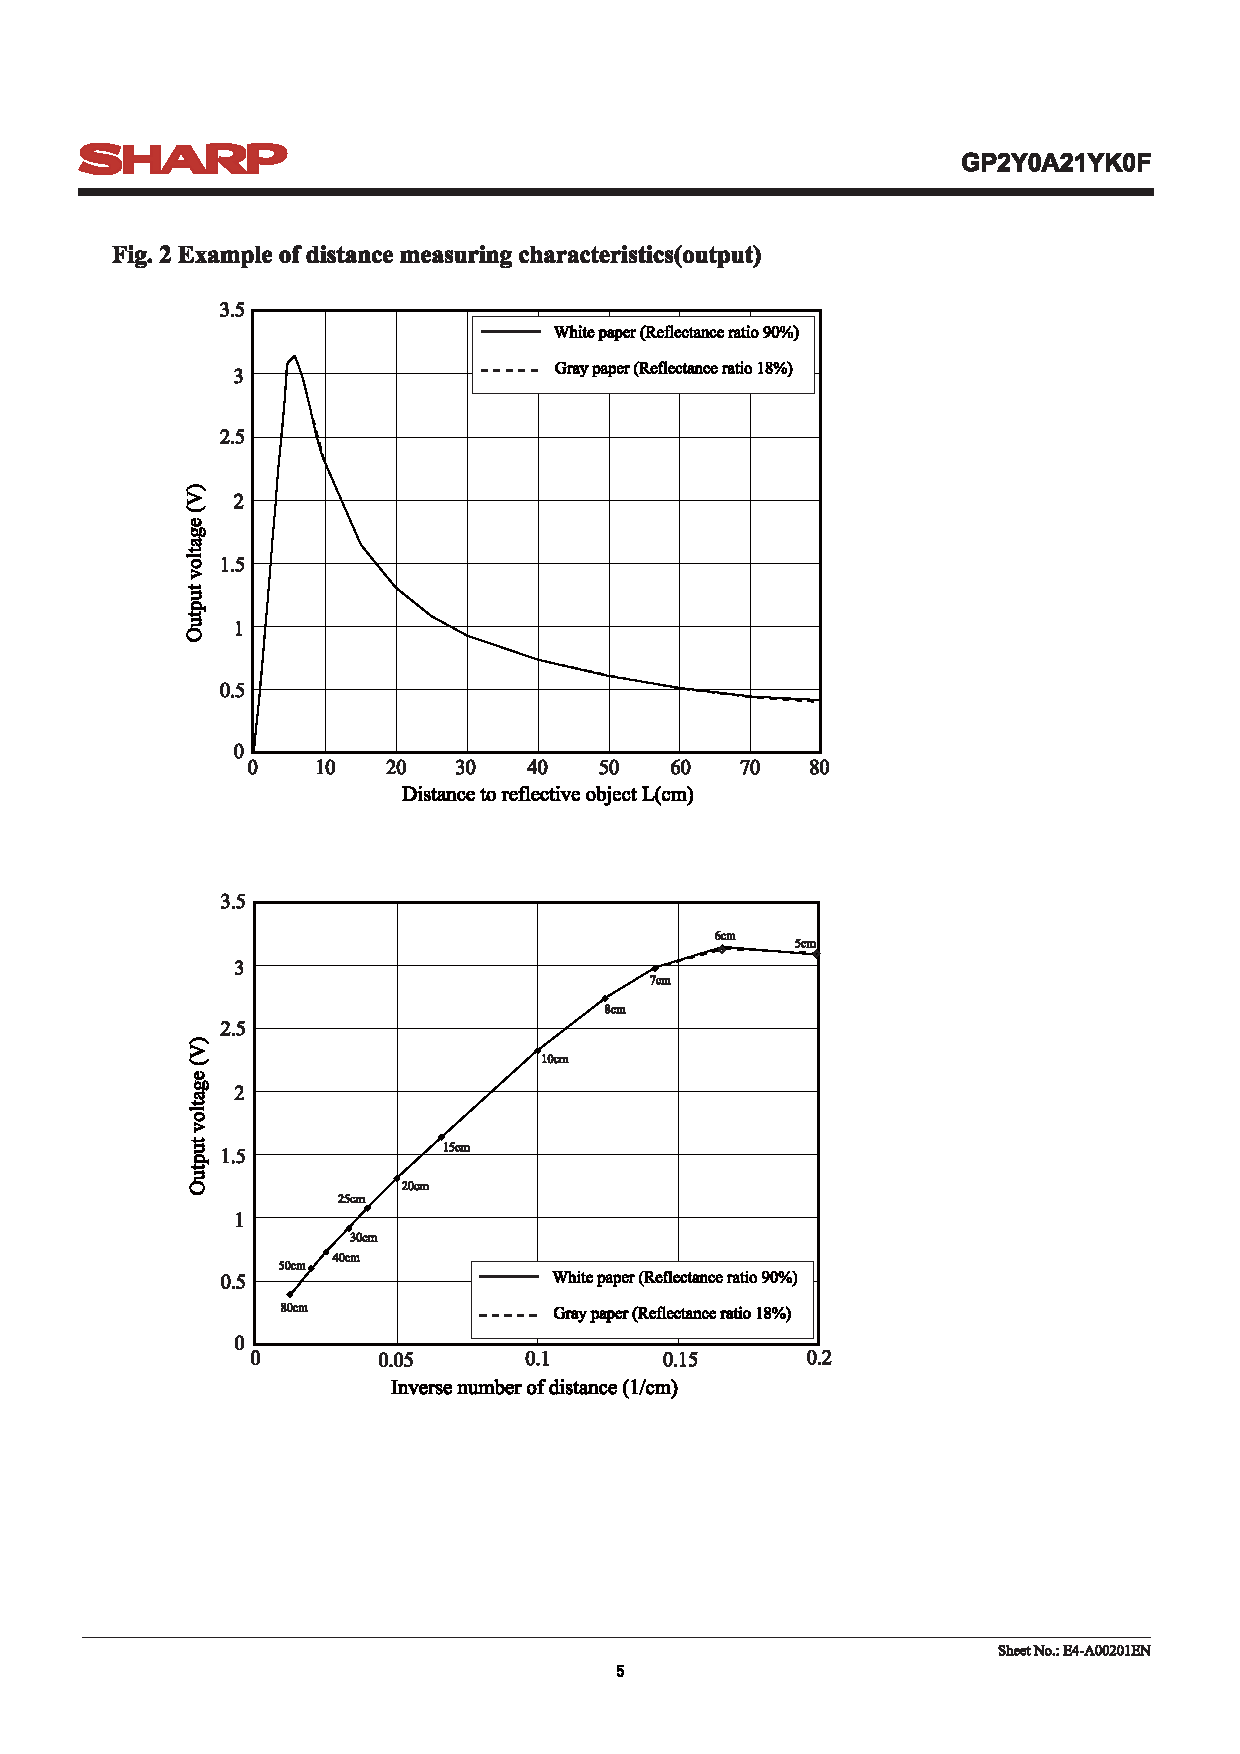
\includegraphics[trim= 3cm 15.8cm 6.5cm 4.8cm,clip,
scale=1]{Figuras/IR_Datasheet_Figure}

	%\begin{tikzpicture}[auto, node distance=2cm, on grid,
%>=latex']%
	
	%\node[anchor=south west,inner sep=0] (image) at (0,0) {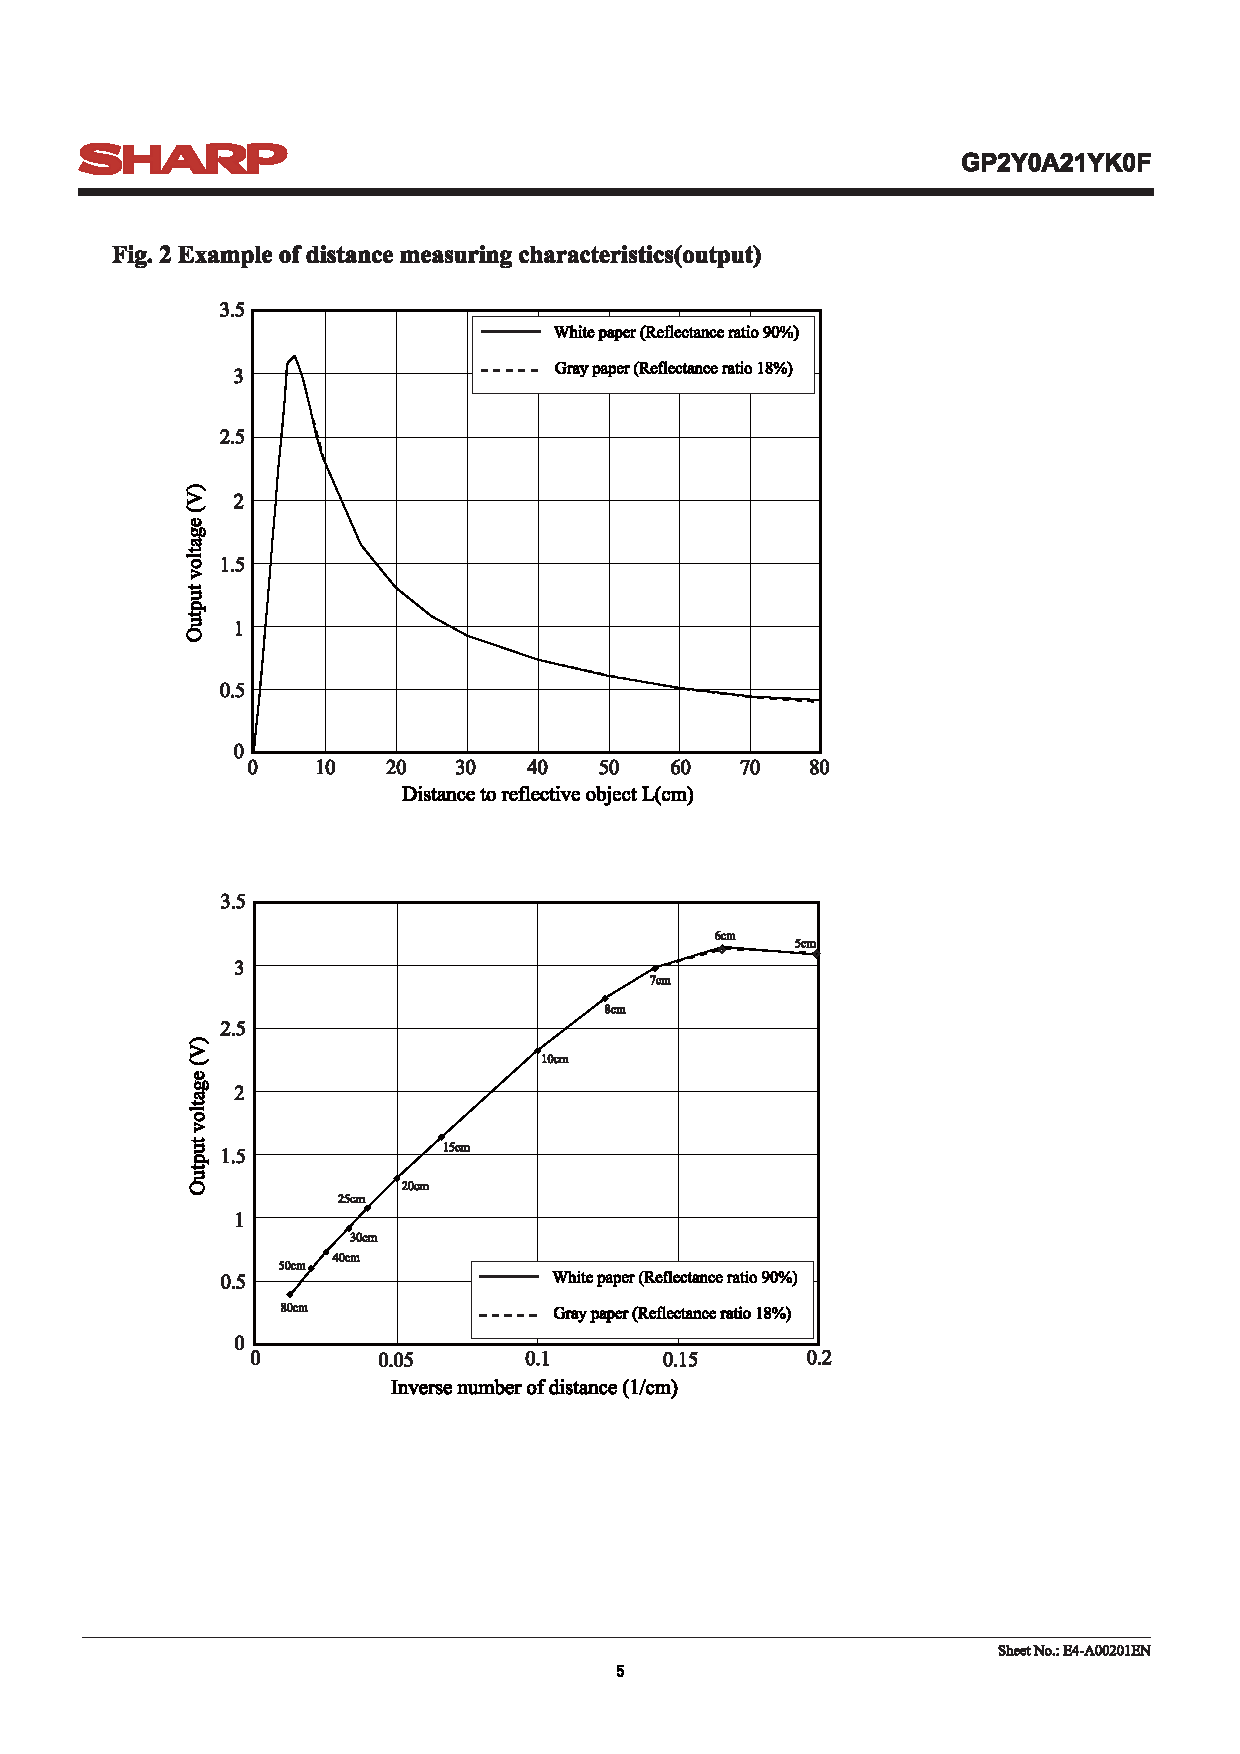
\includegraphics[trim =
%		{3cm 15.8cm 6.5cm 4.8cm}, clip,scale=1]{Figuras/IR_Datasheet_Figure}};
		
%	\node[fill,circle,inner sep=0.1pt, color = red] at (1.29,1.161) {};
%	\node[fill,circle,inner sep=0.1pt, color = red] at (2.525,2.235) {};
	
%	\node[fill,circle,inner sep=0.1pt, color = red] at (1.83,7.75) {};
	
	
%	\node[inner sep = 0 pt, outer sep = 0 pt] (origin) at (1.3,1.15) {};
%	\node[inner sep = 0 pt, outer sep = 0 pt] (teste2) at (2.55,2.25) {};
%	
%	\node[inner sep = 0 pt, outer sep = 0 pt] (P1) at (1.85,7.85) {};
	
	%\draw[-, color = red] (origin) -- (teste2);
	%\draw[-, color = red] (origin) -- (P1);
	
	%\node[] at (0,0) {};
	%\coordinate[] (teste1) {};
	%\coordinate[] (teste2) {};
	
	%\draw[-, color = red] (-18,2) -- (-7,3);
	
%	\end{tikzpicture}


	\textbf{Fonte: \citeonline{datasheet:SensorIR}}
\end{figure}